\chapter{Structure properties and intrinsic defects} \label{ch:results1}  

\label{ch:defects}

\section{Introduction}  

It is important to fully understand the behaviour of intrinsic defects in \zirconia\ before performing studies with dopant ions. In this chapter, intrinsic defects in monoclinic, tetragonal and cubic \zirconia\ are compared and contrasted, including values for formation energy, defect volumes and defect equilibria. Elastic constants, electronic density of states, band gaps and free energies of the non-defective structures are also reported. % because useful material properties may be exploited to improve performance, e.g. by doping with other ions to stabilise one crystal structure. For example, \zirconia\ doped with enough yttrium cations will stabilise the cubic phase and increase the concentration of oxygen vacancies. This would then affect the behaviour of dopant atoms also present in the lattice.

\subsection{Previous work} 

Previous works studying intrinsic defects in the \zirconia\ system have utilised quantum mechanical methods to determine defect formation energies in the monoclinic phase \cite{zheng2007first,foster2002modelling,foster2001structure} and defect equilibria in the tetragonal phase \cite{youssef2012intrinsic}. The cubic phase is mainly studied as a dopant-stabilised system \cite{orera1990intrinsic,jiang2011first}, with few undoped defect studies in the literature \cite{mackrodt1986theoretical,aarhammar2009energetics}. Building upon previous quantum mechanical studies, a comprehensive account of intrinsic defect energies, defect volumes, and defect equilibria for all three common crystal structures of \zirconia\ is provided, using state-of-the-art, accessible methods.

\section{Methodology}
\subsection{Simulation parameters}

As discussed in Chapter \ref{ch:compmethodology}, DFT calculations were performed using CASTEP 8.0 \cite{Clark2005}. Ultra-soft pseudo-potentials were used throughout, employing a 600 eV cut-off energy. The Perdew, Burke and Ernzerhof (PBE) \cite{Perdew1996} parameterisation of the generalised gradient approximation (GGA) was used to describe the exchange correlation functional. A Monkhorst-Pack sampling scheme \cite{Monkhorst1976} was used for Brillouin zone integration, with a minimum \emph{k}-point separation of 0.09 \r{A}\textsuperscript{-1}. The Pulay method for density mixing \cite{Pulay1980} was used to improve convergence of simulations. 

The electrical energy convergence criterion was set to $1\times10^{-6} $ eV. The maximum force between atoms was limited to $1\times10^{-2}$ eV \r{A}\textsuperscript{-1}. A gradient-descent geometry optimisation task was run on the cell until consecutive iterations differed in energy and atomic displacement by less than $1\times10^{-5}$ eV and $5\times10^{-4}$ \r{A}, respectively. 

\subsection{Helmholtz free energy}

As discussed in § \ref{helmholtz_method}, a harmonic approximation was used to determine the temperature dependence of the free energies for the non-defective crystal structures of ZrO$_{2}$. A constant-volume phonon calculation was performed for each structure, from which the vibrational enthalpy $H_{v}(T, V)$ and entropy $S_{v}(T, V)$ contributions to the Helmholtz free energy were calculated up to a temperature of 2500 K in order to cover the temperature range of the three common \zirconia\ phases. The complete Helmholtz free energy $A(T, V)$ was then obtained by including the internal energy $U(V)$ and configurational entropy $S_{conf}$ of the system:
\begin{equation} \label{helmholtz_equation}
A(T, V) = U(V) + H_{v}(T, V) - TS_{v}(T, V) - TS_{conf}
\end{equation}
The calculated free energy was then plotted against temperature to show the relative stability of each phase at different temperatures and the predicted transition points from one phase to another. 

\subsection{Brouwer diagrams}

Using the method outlined in § \ref{brouwer_method}, Brouwer diagrams of the intrinsic defect equilibria for monoclinic, tetragonal and cubic \zirconia\ were generated.  The monoclinic and tetragonal Brouwer diagrams were generated at temperatures of 650 K and 1500 K respectively, corresponding to temperatures at which these phases are thermally stabilised. Defect concentrations are reported in parts/fu (i.e. parts per formula unit \zirconia). The cubic Brouwer diagram was generated at 2000 K despite being thermally stabilised at temperatures greater than 2400 K. This was because such high temperatures resulted in very large intrinsic defect concentrations such that defect behaviour could not be meaningfully examined (the system was completely defective). As discussed in § \ref{dis_form_energy_intrinsic} and § \ref{brouwer_discussion_intrinsic}, issues with modelling cubic \zirconia\ in DFT mean that calculated energy values may become unreliable, but are presented in this thesis for the purpose of completeness.

\section{Non-defective \zirconia}

\subsection{Unit cells}

Having selected and optimised the parameters and functionals, unit cells of \zirconia\ in each phase were fully relaxed at constant pressure and the resulting structures were compared in detail to experimental data. Table \ref{lattice_params} shows the calculated lattice parameters and energy differences between the three \zirconia\ phases. 

\begin{table}[ht] % Unit cell parameters
\onehalfspacing
\centering
\caption[Calculated unit cell parameters for the different crystal structures of \zirconia . Experimental data for pure monoclinic, yttria-stabilised tetragonal and magnesia-stabilised cubic phases at 295 K are shown in parentheses. Energy difference between structures is shown with respect to the cubic phase.]{Calculated unit cell parameters for the different crystal structures of \zirconia . Experimental data for monoclinic, tetragonal and cubic phases at 295 K are shown in parentheses \cite{Howard1988}. Energy difference between structures is shown with respect to the cubic phase.}
\label{lattice_params}
\resizebox{\textwidth}{!}{%
\begin{tabular}{ccccccc}
\hline Phase    & a (\AA) & b (\AA) & c (\AA) & $\beta$ ($\degree$) & Volume (\AA\textsuperscript{3}/fu) & $\Delta$E (eV/fu) \\ \hline
m-\zirconia   &    5.18 (5.15)          &    5.24 (5.21)         &    5.37 (5.32)         & 99.63 (99.23)             &       35.96 (35.22)                 &    -0.215              \\
t-\zirconia &    3.62 (3.61)         &              &    5.28  (5.18)        & 90             &   34.60 (33.75)                      &     -0.105             \\
c-\zirconia        &   5.11 (5.09)           &              &              & 90             &     33.36 (32.97)                   &      N/A     \\ \hline      
\end{tabular}}
\end{table}

The first thing to note is that the correct order of \zirconia\ phases is predicted in the total energy calculations, with monoclinic being the lowest energy phase and cubic being the highest. In addition, the energy difference between phases is small ($<$ 0.1 eV/fu). This is a good indication that the choice of exchange correlation functional can reproduce the energy landscape of the system accurately. This is especially important for when defects are introduced because they may promote stabilisation of one phase over another, and an inaccurate model will not capture this behaviour. In all cases the predicted cell volumes are consistently within approximately 2\% of experimental values. 

\subsection{Elastic constants}

Table \ref{stiffness_tensor} shows the calculated elastic constants for the monoclinic, tetragonal, and cubic phases of \zirconia . The cubic phase has the highest stiffness, likely due to the short Zr-O bond lengths in the energy-minimised structure (Figure \ref{figure:zrobonddistance}). It is expected that at high temperatures where the cubic phase is stable, thermal effects (which are not captured in this model) such as larger interatomic spacings will result in a reduction in stiffness.

\begin{table}[ht] % Elastic constants
\onehalfspacing
\centering
\caption{Elastic constants for different phases of \zirconia\ from DFT calculations.}
\label{stiffness_tensor}
\begin{tabular}{cccc}
\hline
\multirow{2}{*}{\textbf{Elastic Component}} & \multicolumn{3}{c}{\textbf{Stiffness (GPa)}}               \\ \cline{2-4} 
                                            & \textbf{Monoclinic} & \textbf{Tetragonal} & \textbf{Cubic} \\ \hline
$C_{11}$                                         & 338.86        & 334.30               & 523.38    \\
$C_{12}$                                         & 151.80        & 207.30               & 92.93     \\
$C_{13}$                                         & 89.37         & 48.93               & 92.93     \\
$C_{22}$                                         & 348.37        & 334.20               & 523.39    \\
$C_{23}$                                         & 143.04        & 48.93               & 92.93    \\
$C_{33}$                                         & 262.17        & 250.50               & 523.38   \\
$C_{44}$                                         & 76.35         & 9.38                & 61.98    \\
$C_{55}$                                         & 71.65         & 9.38                & 61.98   \\
$C_{66}$                                         & 114.19        & 152.60               & 61.99     \\ \hline
\end{tabular}
\end{table}

The monoclinic and tetragonal phases have similar stiffness along the principal axes, but vary significantly under shearing conditions. In particular, the tetragonal phase exhibits much smaller $C_{44}$ and $C_{55}$ components. This may be attributed to the strong directional anisotropy of the tetragonal phase due to the larger $c$ parameter. 

The bulk modulus ($B$) of each phase was calculated from the elastic constants using the following formulae \cite{Watt1980, Wu2018, wu2017critical}:
\begin{gather}
B_{\ch{monoclinic}} = \frac{1}{9}(C_{11} + C_{22} + C_{33} + 2(C_{12} + C_{13} + C_{23})) \\
B_{\ch{tetragonal}} = \frac{1}{9}(2C_{11} + 2C_{12} + 4C_{13} + C_{33}) \\
B_{\ch{cubic}} = \frac{1}{3}(C_{11} + 2C_{12})
\end{gather}
These yielded bulk modulus values 190.87 GPa, 169.94 GPa and 236.41 GPa for the monoclinic, tetragonal and cubic phases respectively. These compare with experimental values of 201 GPa for monoclinic at 20 $^{\circ}$C \cite{Chan1991}, 176 GPa for tetragonal at room temperature (pressure stabilised between 1-20 GPa) \cite{Bouvier2000} and 201.09 GPa for 10 \% YSZ (cubic) at 300 K \cite{Cai1995}. The monoclinic and tetragonal values are in good agreement with experiment. The cubic phase value is difficult to compare as this phase is always studied with a phase stabilising dopant, thus affecting the measured value.

\subsection{Electronic density of states} 

The electronic density of states for monoclinic, tetragonal and cubic \zirconia\ are generated in a two-step process. First, the non-defective structures are fully relaxed using the geometry optimisation task in CASTEP. This task will also calculate electronic eigenvalues for all k-points and save them to a \texttt{.bands} file. Second, the electronic band data is parsed from the \texttt{.bands} file using the OptaDOS code \cite{Nicholls2012, Morris2014} and the density of states is output to a text file. Further details on using OptaDOS to view the electronic density of states are given in Appendix \ref{castep_scripts}.

The electronic density of states for the three \zirconia\ phase are given in Figure \ref{figure:densityofstates}. In this figure, the valence and conduction bands can clearly be seen at 2-8 eV and 10-15 eV respectively. Most importantly, the energy values of the valence band maximum (VBM) and the conduction band minimum (CBM) for each phase can be obtained from this figure. These values are used to calculate the band gap in the different phases, shown in Figure \ref{table:bandgap} alongside experimental values. The VBM value is also used in the calculation of defect formation energies when electrons are added or removed from a system.

\begin{figure}[ht] % Density of states
\begin{center}
\begin{tikzpicture}
	\begin{axis}
		[width=\linewidth*0.7, xlabel={Energy (eV)}, ylabel={Electronic density of states}, ymin=0, ymax=12, xmin=0, xmax=16, legend style={{draw=}, at={(0.05,0.95)}, anchor=north west, legend columns=1}]
       \addplot[no marks] table [x=mono_x, y=mono_y,]{dat/eDOS.dat}; \addlegendentry{Monoclinic};
       \addplot[no marks, dashed] table [x=tet_x, y=tet_y,]{dat/eDOS.dat}; \addlegendentry{Tetragonal};
       \addplot[no marks, densely dotted] table [x=cubic_x, y=cubic_y,]{dat/eDOS.dat}; \addlegendentry{Cubic};
			\end{axis}
		\end{tikzpicture}
		\caption{Electronic density of states for the different crystal structures of \zirconia\ showing the band gap predicted by DFT.}
		\label{figure:densityofstates}
	\end{center}
\end{figure}

The electronic density of states show that the VBM and CBM energies increase from monoclinic to tetragonal to cubic \zirconia . This means that at the same Fermi level, the total electronic energy will be smallest in the monoclinic phase and largest in the cubic phase. This corresponds to the correct order of thermal stability that is seen in experiments. 

Other features that can be seen are the band gaps of the different phases between 7 and 12 eV. These band gaps are significantly underestimated for each phase (see Table \ref{table:bandgap}), as is typical when using a GGA exchange-correlation functional.

\begin{table}[ht] % Band gap values
\onehalfspacing
\centering
\caption[Experimentally determined band gaps alongside values calculated from DFT simulations for each crystal structure of zirconia.]{Experimentally determined band gaps alongside values calculated from DFT simulations for each crystal structure of zirconia. Experimental values taken from \cite{French1994}.}
\begin{tabular}{ccc}
{\bf }                                       & \multicolumn{2}{c}{{\bf Band gap (eV)}}      \\ \hline
\multicolumn{1}{c}{{\bf Crystal Structure}} & \multicolumn{1}{c}{{\bf Expt.}} & {\bf DFT} \\ \hline
\multicolumn{1}{c}{Monoclinic}              & \multicolumn{1}{c}{5.83}        & 3.45      \\
\multicolumn{1}{c}{Tetragonal}              & \multicolumn{1}{c}{5.78}        & 4.00      \\
\multicolumn{1}{c}{Cubic}                   & \multicolumn{1}{c}{6.10}         &   3.55 \\ \hline
\label{table:bandgap}
\end{tabular}
\end{table}

DFT studies of the monoclinic phase have given a band gap of 3.19 eV when using an LDA \cite{Foster2002} and 3.20 eV when using a GGA \cite{Jaffe2005}. In the tetragonal phase, two GGA-DFT studies calculated band gaps of 4.21 eV \cite{Eichler2001} and 3.55 eV \cite{Jaffe2005}. The band gap in the cubic phase has been calculated in a GGA-DFT study as 2.95 eV \cite{Jaffe2005}. An early ab initio study using a LDA also reported band gaps of 8 eV and 7 eV for tetragonal and cubic ZrO$_{2}$, respectively \cite{morinaga1983electronic}. One study using an ab initio linear combination of atomic orbitals (LCAO) method calculated band gaps of 4.51 eV, 4.11 eV and 3.84 eV for the monoclinic, tetragonal and cubic phases respectively \cite{Zandiehnadem1988}.

All of these studies highlight the difficulty in accurately modelling electronic exchange and correlation behaviour in ZrO$_{2}$. The smaller band gaps calculated in this thesis mean that concentrations of electronic defects will be overestimated because their formation energies are proportional to the size of the band gap. 

\subsection{Helmholtz energies}

The Helmholtz free energy results (Figure \ref{Figure:helmholtz}) predicted the correct order of crystal structure stability at low temperature (monoclinic \textrightarrow tetragonal \textrightarrow cubic). A transition from the monoclinic to tetragonal crystal structure is predicted at 390K, but no further transition is seen from tetragonal to cubic. This significantly underestimates the experimental monoclinic \textrightarrow tetragonal transition temperature of 1180 $^{\circ}$C (see Figure \ref{figure:hysteresis_monotet}). The low phase transition temperature may be due to both the kinetic barrier \cite{bansal1972martensitic,bansal1974martensitic}, and the inability of the constant volume harmonic model to take into account the effects of thermal expansion. 

\begin{figure}[ht] % Helmholtz
\begin{center}
\begin{tikzpicture}
	\begin{axis}
		[width=\linewidth*0.7, xlabel={Temperature (K)}, ylabel={Helmholtz free energy (eV)}, ymin=-28, ymax=-10, xmin=0, xmax=3000, legend style={{draw=}, at={(0.95,0.95)}, anchor=north east, legend columns=1}]
		\addplot[no marks] table [x=temperature, y=monoclinic,]{dat/helmholtz.dat}; \addlegendentry{Monoclinic};
        \addplot[no marks, dashed] table [x=temperature, y=tetragonal, ]{dat/helmholtz.dat}; \addlegendentry{Tetragonal};
        \addplot[no marks, densely dotted, black] table [x=temperature, y=cubic,]{dat/helmholtz.dat}; \addlegendentry{Cubic};
			\end{axis}
		\end{tikzpicture}
		\caption{Helmholtz free energy as a function of temperature for the monoclinic, tetragonal, and cubic crystal structures of \zirconia .}
		\label{Figure:helmholtz}
	\end{center}
\end{figure}

The lack of an observed transition to the cubic phase may further indicate an inability to accurately simulate the high-temperature phase using DFT techniques, possibly owing to finite-size effects which are known to affect ZrO$_{2}$ in particular \cite{burr2017importance}. When proceeding to model certain defects (see § \ref{bound_defect}), it was discovered that the cubic phase did indeed exhibit instabilities which yielded anomalous energy values. These results, in addition to the lack of experimental evidence showing pure cubic ZrO$_{2}$ in the internal oxide layer of Zr claddings, led to the decision to focus further studies only on the monoclinic and tetragonal phases.

\section{Defective \zirconia} \label{dis_form_energy_intrinsic}

\subsection{Formation energies}

Calculated point defect formation energies are provided and discussed below as a function of the Fermi level, defined as the electrochemical potential above the energy of the valence band maximum (VBM). Formation energies are plotted up to a Fermi level of 6 eV in order to span the entire experimental band gap of \zirconia . Only the defects with the lowest formation energies at each Fermi level are shown.

\subsubsection{Monoclinic}

Oxygen vacancies in the monoclinic phase are shown in Figure \ref{figure:monovacancies} for both the III and IV coordinated oxygen atoms. At Fermi levels between 0 and 3 eV, formation of \ch{V_{O}^{**}} defects is expected, with III coordinated oxygen atoms having formation energies 0.6 eV lower. This energy difference between the two types of oxygen vacancy is substantial, and since both are anion sites of the same charge, this suggests that the defect size is the main reason for the difference in energy. In this case, a vacancy at the III oxygen site is larger defect than at the IV oxygen site (see § \ref{defect_volumes_r1} for defect volumes), and the negative energies reveal that the non-defective monoclinic structure is too large at low Fermi levels. At Fermi levels above 3 eV, \ch{V_{O}^{x}} defects become the most favourable at both oxygen sites, with almost the same formation energy (0.9 eV). The defect with the smallest formation energy switches from \ch{V_{O}^{**}} to \ch{V_{O}^{x}} as the Fermi level is increased. The absence of \ch{V_{O}^{*}} defects is due to the relatively unfavourable electronic state imposed in the lattice with this defect configuration. This could be because of the suboptimal orbital occupancy in the surrounding ions when a single electron is missing rather than two.

\begin{figure}[ht] % Mono vacancies Fermi level
\begin{center}
\begin{tikzpicture}
	\begin{axis}
		[width=11cm, xlabel={Fermi level $\mu_{e}$ (eV)}, ylabel={Formation energy (eV) per \zirconia\ }, ymin=-10, ymax=18, xmin=0, xmax=6, legend style={{draw=}, at={(0.95,0.95)}, anchor=north east, legend columns=1}]
		\addplot[no marks, blue] table [x=ZRmono1, y=ZRmono2,]{dat/vacancies.dat}; \addlegendentry{\ch{V_{Zr}}} \node at (3,10) {-4};
        \addplot[no marks, red, dashed] table [x=O3mono1, y=O3mono2,]{dat/vacancies.dat}; \addlegendentry{\ch{V_{O}} (III)} \node at (1.0,-1.5) {+2};
        \addplot[no marks, red] table [x=O4mono1, y=O4mono2,]{dat/vacancies.dat}; \addlegendentry{\ch{V_{O}} (IV)};
			\end{axis}
		\end{tikzpicture}
		\caption{Monoclinic phase formation energies of intrinsic vacancy defects as a function of Fermi level. Gradient indicates defect charge. Oxygen coordination number shown in legend.}
		\label{figure:monovacancies}
	\end{center}
\end{figure}



\subsubsection{Tetragonal}

XXX

\begin{figure}[ht] % Tet vacancies Fermi level
\begin{center}
\begin{tikzpicture}
	\begin{axis}
		[width=11cm, xlabel={Fermi level $\mu_{e}$ (eV)}, ylabel={Formation energy (eV) per \zirconia\ }, ymin=-10, ymax=18, xmin=0, xmax=6, legend style={{draw=}, at={(0.95,0.95)}, anchor=north east, legend columns=1}]
		\addplot[no marks, blue] table [x=ZRtet1, y=ZRtet2,]{dat/vacancies.dat}; \addlegendentry{Zr};
        \addplot[no marks, red] table [x=Otet1, y=Otet2,]{dat/vacancies.dat}; \addlegendentry{O};
			\end{axis}
		\end{tikzpicture}
		\caption{Tetragonal phase formation energies of intrinsic vacancy defects as a function of Fermi level. Gradient indicates defect charge.}
		\label{figure:tetvacancies}
	\end{center}
\end{figure}

\subsubsection{Cubic}

XXX

\begin{figure}[ht] % Cubic vacancies Fermi level
\begin{center}
\begin{tikzpicture}
	\begin{axis}
		[width=11cm, xlabel={Fermi level $\mu_{e}$ (eV)}, ylabel={Formation energy (eV) per \zirconia\ }, ymin=-10, ymax=18, xmin=0, xmax=6, legend style={{draw=}, at={(0.95,0.95)}, anchor=north east, legend columns=1}]
		\addplot[no marks, blue] table [x=ZRcubic1, y=ZRcubic2,]{dat/vacancies.dat}; \addlegendentry{Zr};
        \addplot[no marks, red] table [x=Ocubic1, y=Ocubic2,]{dat/vacancies.dat}; \addlegendentry{O};
			\end{axis}
		\end{tikzpicture}
		\caption{Cubic phase formation energies of intrinsic vacancy defects as a function of Fermi level. Gradient indicates defect charge.}
		\label{figure:cubicvacancies}
	\end{center}
\end{figure}

\subsection{Frenkel and Schottky defects}

Formation energies for Frenkel and Schottky defects were calculated in either a \emph{bound} or \emph{isolated} configuration. A bound defect means that the entire defect (interstitial + vacancy for a Frenkel defect or three vacancies for a Schottky defect) is modelled inside a single supercell. An isolated defect means that the formation energy was calculated from the constituent point defects (individual vacancy or interstitial defects). Both of these methods were used for completeness and because the bound defects include binding energy contributions. Bound and isolated defects are described in more detail below.

\subsubsection{Isolated Frenkel defects}

Zr and O Frenkel pair defect formation energies were determined via point defect DFT calculations for the three structures. The formation energies of the isolated Frenkel defect pairs were defined as: % Interstitial iodine defects were simulated in the neutral charge state at different interstitial sites in each phase. The incorporation energy of these defects, assuming a perfect lattice, was calculated using Equation \ref{equation_incorporation}:
\begin{equation}
\label{equation_frenkel}
E_{Frenkel} = E_{DFT}(V^{q}_{X}) + E_{DFT}(X^{-q}_{i}) - 2E_{DFT}(ZrO_2)% - \frac{E_{I_2}}{2}
\end{equation}

where $X$ is either Zr or O, $E_{DFT}(V^{q}_{X})$ is the energy of a supercell of \zirconia\ containing a single vacancy of charge $q$, $E_{DFT}(X^{-q}_{i})$ is the energy of a supercell of \zirconia\ containing a single interstitial with opposing charge $-q$, and $E_{DFT}(ZrO_2)$ is the energy of the non-defective supercell. Charges ranged from the fully charged case (+2 for oxygen vacancies, -4 for zirconium vacancies) to neutral. The interstitial sites, shown in Table \ref{table:interstitials}, were chosen based on standard vacant Wyckoff positions in each crystal structure \cite{theo1996international}.  In the case of oxygen vacancies in monoclinic \zirconia , a defect energy was obtained for both the (III) and (IV) co-ordinated oxygen sites, with the lowest energy value being used in the calculation of the Frenkel defect energy.

\begin{table}[ht] % Wyckoff positions of interstitials
\onehalfspacing
\centering
\caption{Wyckoff positions of interstitial sites used for each crystal structure.}
\label{table:interstitials}
\begin{tabular}{lcc}
\hline
\hspace{0.7 cm} {\bf Crystal Structure} \hspace{0.7 cm}                              & \hspace{0.7 cm} {\bf Interstitial Sites} \hspace{0.7 cm}                                               \\ \hline
\multicolumn{1}{c}{\textbf{Monoclinic}}              & $2a$, $2b$, $2c$, $2d$ \\
\multicolumn{1}{c}{\textbf{Tetragonal}}            & $2b$, $8e$                                   \\
\multicolumn{1}{c}{\textbf{Cubic}}       & $24d$, $4b$                                          \\ \hline
\end{tabular}
\end{table}

The isolated defect formation energies reported in Table \ref{isolated_defects} indicate that fully-charged Schottky defects have the lowest formation energy per atom (most energetically favourable) in all phases, followed by oxygen Frenkel defects and then zirconium Frenkel defects. A trend is seen where the high-temperature phases result in lower formation energies for both Schottky and oxygen Frenkel defects, whereas zirconium Frenkel defects have similar formation energies in all three phases. The formation energy of a neutral oxygen vacancy-oxygen atom Frenkel pair is calculated as 7.52 eV, which is in good agreement with another DFT study (using the LDA) in the literature which calculated the formation energy as 7.3 eV \cite{Foster2002}. Theoretical calculations of the oxygen Frenkel formation energy in cubic \zirconia\ gave an energy of 9.1 eV \cite{mackrodt1986theoretical}, compared to 8.48 eV in this study for the neutral oxygen Frenkel defect in the cubic phase. Ab initio calculations of zircon, which has a tetragonal crystal structure, also yielded a formation energy of 7.3 eV \cite{Crocombette1999}.

It has been suggested that the relatively small cation size leads to defect structures where oxygen vacancies are favoured over interstitial defects \cite{dwivedi1990computer}. As the zirconium ion is too small to maintain a strong 8-fold bond coordination with its neighbouring oxygen ions, the introduction of oxygen vacancies (which have the added effect of reducing cell volume) will have a stabilising effect.

\begin{table}[ht] % Isolated formation energies
\onehalfspacing
\centering
\caption{Formation energies in eV of isolated \zirconia\ defects.}
\label{isolated_defects}
\begin{tabular}{cccll}
\hline
\multirow{2}{*}{\textbf{Defect}}                      & \multirow{2}{*}{\textbf{Equation}}                                        & \multicolumn{3}{c}{\textbf{Formation Energy (eV)}} \\ \cline{3-5}
	&	& \multicolumn{1}{l}{Monoclinic} & Tetragonal & Cubic \\ \hline
\multirow{5}{*}{\textbf{Zr Frenkel}} & \ch{Zr_{Zr}^{x}} $\rightarrow$ \ch{V_{Zr}^{''''}} + \ch{Zr_{i}^{****}}              & 5.43 & 5.64 & 5.61                             \\
                                     & \ch{Zr_{Zr}^{x}} $\rightarrow$ \ch{V_{Zr}^{'''}} + \ch{Zr_{i}^{***}}               & 8.70 & 8.94 & 8.48                            \\
                                     & \ch{Zr_{Zr}^{x}} $\rightarrow$ \ch{V_{Zr}^{''}} + \ch{Zr_{i}^{**}}                & 12.12 & 12.06 & 11.63                             \\
                                     & \ch{Zr_{Zr}^{x}} $\rightarrow$ \ch{V_{Zr}^{'}} + \ch{Zr_{i}^{*}}                & 16.02 &	15.70 &	13.32                             \\
                                     & \ch{Zr_{Zr}^{x}} $\rightarrow$ \ch{V_{Zr}^{x}} + \ch{Zr_{i}^{x}}                  & 20.56	& 20.09 &	18.17                            \\ \hline
\multirow{3}{*}{\textbf{O Frenkel}}  & \ch{O_{O}^{x}} $\rightarrow$ \ch{V_{O}^{**}} + \ch{O_{i}^{''}}                   & 4.46 &	4.00 & 	3.73 \\
                                     & \ch{O_{O}^{x}} $\rightarrow$ \ch{V_{O}^{*}} + \ch{O_{i}^{'}}                   & 6.43	& 6.59 &	7.06                             \\
                                     & \ch{O_{O}^{x}} $\rightarrow$ \ch{V_{O}^{x}} + \ch{O_{i}^{x}}                     & 7.52 & 7.45 &	8.48                             \\ \hline
\multirow{3}{*}{\textbf{Schottky}}   & $\varnothing$ $\rightarrow$ \ch{V_{Zr}^{''''}} + 2\ch{V_{O}^{**}} & 5.12 &	3.78	& 1.75                            \\
                                     & $\varnothing$ $\rightarrow$ \ch{V_{Zr}^{''}} + 2\ch{V_{O}^{*}} & 11.35 &	10.83 &	9.62                             \\
                                     & $\varnothing$ $\rightarrow$ \ch{V_{Zr}^{x}} + 2\ch{V_{O}^{x}}   & 18.55 &	18.23 &	17.07  \\ \hline                          
\end{tabular}
\end{table}

\subsubsection*{Bound Frenkel Defects}

Bound Zr and O Frenkel defect formation energies were calculated from DFT energies of supercells where a single ion was moved from its lattice site to an interstitial site. The formation energies of the bound Frenkel defect pairs were defined as:
\begin{equation}
\label{equation_frenkel_bound}
E_{BoundFrenkel} = E_{DFT}(BoundFrenkel) - E_{DFT}(ZrO_2)% - \frac{E_{I_2}}{2}
\end{equation}
where $E_{DFT}(BoundFrenkel)$ is the energy of a supercell of \zirconia\ containing both a vacancy and interstitial defect of the same ion. The two defects were placed as far apart in the supercell as possible (7-8 \r{A}) to avoid recombination. The interstitial defect is assumed to fully compensate the charge of the vacancy defect, resulting in no overall charge on the supercell. The number and type of ions in the defective and non-defective supercell are the same, requiring no further steps to calculate the formation energy. The formation energies calculated for these defects in each crystal structure are presented in Table \ref{table:bound_defects}.

\subsubsection*{Isolated Schottky Defects}

Three Schottky energies were calculated for each structure, corresponding to fully charged, partially charged, and uncharged point defect energies. The Schottky formation energy was defined as:
\begin{equation}
\label{equation_schottky}
E_{Schottky} = E_{DFT}(V^{-2q}_{Zr}) + 2E_{DFT}(V^{q}_{O}) -\frac{3(n-1)}{n}E_{DFT}(ZrO_2)% - \frac{E_{I_2}}{2}
\end{equation}
where $n$ denotes the number of atoms in the supercell, $V^{q}_{O}$ denotes an oxygen vacancy with charge $q$, where $q$ varies from 2 to 0. This form maintains both the mass and charge balance of the Schottky defect description for \zirconia :
\begin{equation}
\label{generic_schottky}
Zr^{x}_{Zr} + 2O^{x}_{O} = V^{-2q}_{Zr} + 2V^{q}_{O} + ZrO_{2}
\end{equation}
This implies a rearrangement rather than complete removal of ions from the system. As with the Frenkel defects, the lowest energy vacancy energies were used to calculate Schottky formation energies. While there are multiple configurations of Schottky defects, such nuance cannot be accurately represented through a sum of individual vacancy defect energies. The values presented for Schottky defect formation energies should therefore be considered the lower bound for defect formation. 

\subsubsection{Bound Schottky Defects}

Bound Schottky defects were modelled in a supercell of \zirconia\ by removing one Zr and two O atoms, in one of several possible nearest neighbour configurations as shown in Figures \ref{figure:monoschottky}, \ref{figure:tetschottky} and \ref{figure:cubicschottky}. For the monoclinic phase, Schottky defects included one threefold and one fourfold coordinated oxygen to maintain equal amounts of each oxygen type in the supercell.

\begin{figure}[ht] % Tet Zr centre
\centering
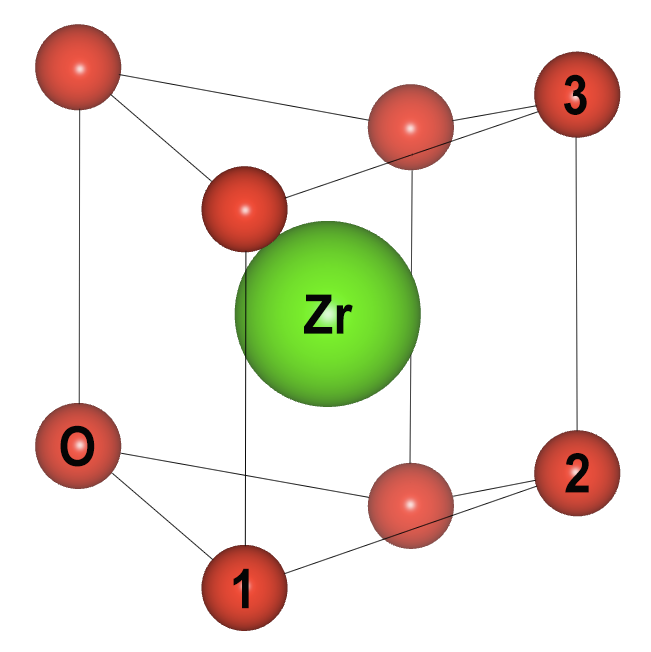
\includegraphics[width=8cm]{images/zr_centre_tet.png}
\caption{Zirconium centre  cell showing nearest oxygen atoms in tetragonal \zirconia. Schottky trios indicated by oxygen enumeration with Zr, O and a second oxygen in either the 1\textsuperscript{st}, 2\textsuperscript{nd} or 3\textsuperscript{rd} nearest neighbour with respect to the initial oxygen. Zirconium atoms are shown in green and oxygen atoms in red.}
\label{figure:tetschottky}
\end{figure}

\begin{figure}[ht] % Cubic Zr centre
\centering
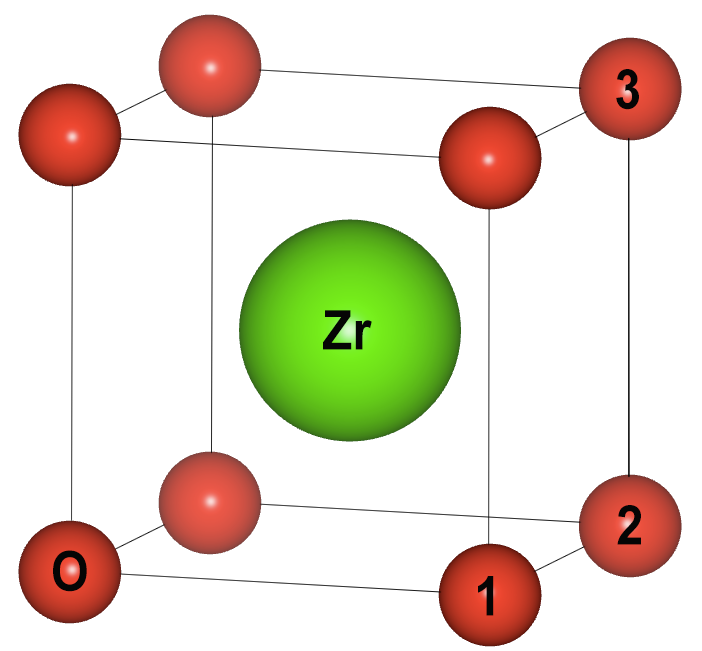
\includegraphics[width=8cm]{images/sd_cubic_zro2.png}
\caption{Zirconium centre cell showing nearest oxygen atoms in cubic \zirconia. Schottky trios indicated by oxygen enumeration with Zr, O and a second oxygen in either the 1\textsuperscript{st}, 2\textsuperscript{nd} or 3\textsuperscript{rd} nearest neighbour with respect to the initial oxygen.. Zirconium atoms are shown in green and oxygen atoms in red.}
\label{figure:cubicschottky}
\end{figure}

Charge neutrality is maintained by the removal of a stoichiometric unit, therefore these defects were defined as neutral tri-vacancies (NTVs). The NTV formation energy was defined as:
\begin{equation}
\label{equation_NTV}
E_{NTV} = E_{DFT}(NTV) - \frac{n-3}{n}E_{DFT}(ZrO_2)% - \frac{E_{I_2}}{2}
\end{equation}
Where $E_{DFT}(NTV)$ is the energy of a supercell containing the NTV defect. As the defective supercell contains three fewer ions than the non-defective cell, the energy of the non-defective cell was adjusted by a proportional factor in our calculation. This form maintains both mass and charge balance of the Schottky defect description for \zirconia\ described in Equation \ref{generic_schottky}.

\subsection{Defect Volumes} \label{defect_volumes_r1}

Tables \ref{defect_volumes_raw} and \ref{defect_volumes_clusters_isolated} show the calculated point defect and cluster defect volumes respectively. The Frenkel and Schottky defect volumes are calculated from the sum of the relevant point defects that would result in an overall neutral charge, with clusters of fully-charged point defects being the expected defect structures in a real material.

\begin{table}[ht!] % Isolated defect volumes
\onehalfspacing
\centering
\caption{Individual point defect volumes in the three \zirconia\ structures.}
\label{defect_volumes_raw}
\begin{tabular}{cccc}
\hline
                      & \multicolumn{3}{c}{\textbf{Defect volume relative to non-defective cell (\r{A}\textsuperscript{3})}}  \\ \cline{2-4} 
\textbf{Defect}       & \textbf{Monoclinic} & \hspace{1cm} \textbf{Tetragonal} & \textbf{Cubic} \\ \hline
\ch{V_{Zr}^{''''}}             & 55.95             & 88.93            & 48.47         \\
\ch{V_{Zr}^{'''}}             & 42.48             &         51.08     &     36.94      \\
\ch{V_{Zr}^{''}}            & 29.90             &  34.28            &     25.93           \\
\ch{V_{Zr}^{'}}             & 17.10             &  18.43            &     15.08           \\
\ch{V_{Zr}^{x}}              & 4.06             &  4.70            &    4.32       \\
\ch{Zr_{i}^{****}}             & -34.62            & -41.94            & -27.34       \\
\ch{Zr_{i}^{***}}             &  -22.76           &	-27.74 		  &	-16.95         \\
\ch{Zr_{i}^{**}}             &  -11.79 	        &	-12.02 		  &	-6.24          \\
\ch{Zr_{i}^{*}}            &  2.68			& -0.02 		  & 	4.69             \\
\ch{Zr_{i}^{x}}              &  15.94		 	& 13.40	 		  & 15.97         \\
\ch{V_{O}^{**}} {[}4coord{]} & -22.52            & -40.45            & -22.76       \\
\ch{V_{O}^{*}} {[}4coord{]} &  -12.41           &    -19.53         &     -12.19           \\
\ch{V_{O}^{x}} {[}4coord{]}  &  -0.69          &  -2.80           &      -1.11          \\
\ch{V_{O}^{**}} {[}3coord{]} & -26.13            &                     &                \\
\ch{V_{O}^{*}} {[}3coord{]} &  -14.42           &                     &                \\
\ch{V_{O}^{x}} {[}3coord{]}  &   -1.71          &                     &                \\
\ch{O_{i}^{''}}              & 27.01             & 40.00              & 28.58        \\
\ch{O_{i}^{'}}              &  15.36            &    24.56         &  16.30              \\
\ch{O_{i}^{x}}               & 2.66             &    11.06          &   8.95        \\ \hline
\end{tabular}
\end{table}

\begin{table}[ht] % Isolated Frenkel + Schottky volumes
\onehalfspacing
\centering
\caption{Defect volumes of Frenkel and Schottky defects in the three \zirconia\ structures calculated from individual point defects.}
\label{defect_volumes_clusters_isolated}
\begin{tabular}{cccc}
\hline
                      & \multicolumn{3}{c}{\textbf{Defect volume relative to non-defective cell (\r{A}\textsuperscript{3})}}  \\ \cline{2-4} 
\textbf{Defect}       & \textbf{Monoclinic} & \hspace{1cm} \textbf{Tetragonal} & \textbf{Cubic} \\ \hline
\ch{V_{Zr}^{''''}} + \ch{Zr_{i}^{****}}          & 21.33	 & 46.99 &	21.13         \\
\ch{V_{Zr}^{'''}} + \ch{Zr_{i}^{***}}          & 19.72 &	23.35 &	20.00      \\
\ch{V_{Zr}^{''}} + \ch{Zr_{i}^{**}}          & 18.11 &	22.25 & 19.69           \\
\ch{V_{Zr}^{'}} + \ch{Zr_{i}^{*}}          & 19.78 &	18.41 &	19.76           \\
\ch{V_{Zr}^{x}} + \ch{Zr_{i}^{x}}          & 19.99 &	18.11 &	20.29       \\
\ch{V_{O}^{**}} + \ch{O_{i}^{''}}           & 0.88 &	-0.45 &	 5.82       \\
\ch{V_{O}^{*}} + \ch{O_{i}^{'}}           &  0.95 &	5.03 &	4.11        \\
\ch{V_{O}^{x}} + \ch{O_{i}^{x}}           &  0.96 &	8.26 &	7.84          \\
\ch{V_{Zr}^{''''}} + 2\ch{V_{O}^{**}}       &  3.70 &	8.03 &	2.94             \\
\ch{V_{Zr}^{''}} + 2\ch{V_{O}^{*}}       &  1.07 &	-4.79 &	 1.56         \\
\ch{V_{Zr}^{x}} + 2\ch{V_{O}^{x}}        & 0.65 &	-0.90 &	 2.09       \\ \hline
\end{tabular}
\end{table}

The fully-charged O Frenkel defect has the smallest defect volume in the tetragonal phase, followed by the monoclinic phase. This can be explained by the relative stiffness of the different phases. Of the nine calculated elastic components of the stiffness tensor shown in table \ref{stiffness_tensor}, seven are smaller in the tetragonal phase compared to monoclinic, and by significant amounts for the $C_{23}$, $C_{44}$ and $C_{55}$ components. In the monoclinic phase, none of the calculated elastic components are below 71 GPa, whereas four of the elastic components in the tetragonal phase are below 50 GPa, making the structure more compliant. The resulting smaller defect volume may then partly explain the lower formation energy of O Frenkel defects in the tetragonal phase, since they impose a smaller strain on the lattice.

The Zr Frenkel defect is significantly larger than the oxygen Frenkel, mostly due to the large positive strain contribution from the zirconium vacancy. The tetragonal phase in particular has a significantly larger fully-charged Zr Frenkel defect, again partly due to the low stiffness of the tetragonal phase. Compared to the O Frenkel defect, these defects are significantly larger and will therefore impose larger strains in the lattice, leading to larger formation energies. 

\subsubsection*{Bound Defects} \label{bound_defect}

The bound defect formation energies shown in Table \ref{table:bound_defects} show that NTV defects, on a per defect atom basis, are the most energetically favourable defects, followed by oxygen and zirconium Frenkel defects respectively. The NTV3 exhibited the smallest formation energy in all three crystal structures, with a single exception of the NTV2 in the cubic phase where a much smaller formation energy was observed due to collapse\footnote{Upon inspecting the output cell, it was found that all the oxygen atoms shifted positions along the [001] direction, becoming more like the tetragonal \zirconia\ structure. The cell size was constrained so the lattice parameters could not be changed, therefore this was not a P4$_{2}$/nmc tetragonal cell.} of the supercell during geometry optimisation. 

\begin{table}[ht] % Bound formation energies
%\setlength{\tabcolsep}{10pt} % Default value: 6pt
\onehalfspacing
\centering
\caption{Formation energies of bound defects in \zirconia.}
\label{table:bound_defects}
\begin{tabular}{cccc}
\hline
\multirow{2}{*}{\textbf{Defect}} & \multicolumn{3}{c}{\textbf{Formation Energy (eV)}} \\ \cline{2-4} 
 & \textbf{Monoclinic} & \textbf{Tetragonal} & \textbf{Cubic} \\ \hline
\textbf{O Frenkel} & 4.12 & 4.03 & 6.44 \\
\textbf{Zr Frenkel} & 8.42 & 7.86 & 6.33 \\
\textbf{NTV1} & 5.23 & 3.58 & 2.70 \\
\textbf{NTV2} & 5.14 & 4.23 & 0.18 \\
\textbf{NTV3} & 4.66 & 3.36 & 2.41 \\ \hline
\end{tabular}
\end{table}

The symmetry of cubic ZrO$_{2}$ has previously been reported to sometimes break when relaxing supercells with interstitial oxygen defects \cite{samanta2010thermodynamic}. However, reports of Schottky defect clusters breaking cubic symmetry in \zirconia\ have not been found in the literature. Later studies by Burr \emph{et al}. have shown that the energies of NTVs calculated in MO$_{2}$ cubic fluorite structures is highly sensitive to the size of the supercell, with larger errors found when using smaller supercells \cite{burr2017importance}. It was also found that the symmetry of cubic ZrO$_{2}$ could not be retained during relaxation in large supercells (324 and 768 atoms) due to the stability of the monoclinic phase. Cubic supercells with 96 atoms are studied in this thesis, and while cubic symmetry of \zirconia\ can be retained at this size, the instability of the phase when introducing defect clusters puts the bound defect energies into question.

\subsection{Defect equilibria} \label{brouwer_discussion_intrinsic}

\subsubsection*{Monoclinic}

The monoclinic Brouwer diagram (Figure \ref{figure:mono_intrinsic_brouwer}) predicts that at 650 K, intrinsic defects will be present at very low (\textless 10 ppb \zirconia ) concentrations. This is typical of defect behaviour in a ceramics at temperatures far below their melting points \cite{kingery1997physical,ball2006computer}. At oxygen pressures below $10^{-20}$ atm, the major defects are \ch{e^{'}} and \ch{h^{*}} which fully charge-compensate each other. As the oxygen pressure increases, \ch{V_{Zr}^{'''}} defects become more numerous and overtake \ch{e^{'}} defects as the dominant negatively charged defect. The greater charge magnitude of the \ch{V_{Zr}^{''''}} defects force the formation of more \ch{h^{*}} defects as these are the easiest positively charged defects which can be produced to achieve charge neutrality (i.e. \ch{V_{O}^{**}} and \ch{Zr_{i}^{****}} defects require too much energy to produce at high oxygen pressures). \ch{O_{i}^{x}} defects are also present at high oxygen pressures, but these do not affect the concentrations of charged defects.

%Fully-charged zirconium vacancies, charge-compensated by holes, are the major defect type we expect to observe at $p_{O_{2}}$ \textgreater $10^{-15}$ atm. Below this, only \ch{e^{'}} defects compensated by electron hole defects are expected. 

%We briefly see increased concentrations of uncharged oxygen interstitial defects at very high levels of $p_{O_{2}}$.
%The intrinsic defect equilibria are shown in Brouwer diagrams in Figures \ref{figure:mono_intrinsic_brouwer}, \ref{figure:tet_intrinsic_brouwer} and \ref{figure:cubic_intrinsic_brouwer}. The monoclinic phase exhibits the smallest overall concentration of intrinsic defects due to the low temperature (650 K) relative to the other tetragonal (1500 K) and cubic (XXX K) phases.

\begin{figure}[ht] % Mono intrinsic Brouwer
\begin{center}
\begin{tikzpicture}
	\begin{axis}
		[width=\linewidth*0.7, xlabel={\ch{log_{10}}($p_{O_{2}}$) (atm)}, ylabel={\ch{log_{10}}([D]) (per f.u.)}, ymin=-18, ymax=0, xmin=-35, xmax=0, legend style={{draw=}, at={(0.40,0.94)}, anchor=north west, legend columns=4, nodes={scale=1, transform shape}}]
        \addplot[no marks, draw=blue!70!black] table [x=pO2, y=electrons,]{dat/intrinsic_mono.dat}; \addlegendentry{\ch{e^{'}}}; \node at (-5.5,-12.2) {\ch{e^{'}}};
        \addplot[no marks, draw=red!85!black] table [x=pO2, y=holes,]{dat/intrinsic_mono.dat}; \addlegendentry{\ch{h^{\textperiodcentered}}}; \node at (-4.5,-8) {\ch{h^{\textperiodcentered}}};
        \addplot[no marks, draw=black!70!green] table [x=pO2, y=VO{2},]{dat/intrinsic_mono.dat}; \addlegendentry{\ch{V_{O}^{\textperiodcentered\textperiodcentered}}}; \node at (-33,-16.5) {\ch{V_{O}^{\textperiodcentered\textperiodcentered}}};
%         \addplot[no marks, draw=black!55!green] table [x=pO2, y=VO{1},]{dat/intrinsic_mono.dat}; \addlegendentry{\ch{V_{O}^{*}}};
%         \addplot[no marks, draw=black!30!green] table [x=pO2, y=VO{0},]{dat/intrinsic_mono.dat}; \addlegendentry{\ch{V_{O}^{x}}};
        \addplot[no marks, draw=yellow!85!blue] table [x=pO2, y=VM{-4},]{dat/intrinsic_mono.dat}; \addlegendentry{\ch{V_{Zr}^{''''}}}; \node at (-5,-10.5) {\ch{V_{Zr}^{''''}}};
%         \addplot[no marks, draw=yellow!75!blue] table [x=pO2, y=VM{-3},]{dat/intrinsic_mono.dat}; \addlegendentry{\ch{V_{Zr}^{'''}}};
%         \addplot[no marks, draw=yellow!65!blue] table [x=pO2, y=VM{-2},]{dat/intrinsic_mono.dat}; \addlegendentry{\ch{V_{Zr}^{''}}};
%         \addplot[no marks, draw=yellow!55!blue] table [x=pO2, y=VM{-1},]{dat/intrinsic_mono.dat}; \addlegendentry{\ch{V_{Zr}^{'}}};
%         \addplot[no marks, draw=yellow!45!blue] table [x=pO2, y=VM{0},]{dat/intrinsic_mono.dat}; \addlegendentry{\ch{V_{Zr}^{x}}};
         %\addplot[no marks, draw=red!60!yellow] table [x=pO2, y=Oi{-2},]{dat/intrinsic_mono.dat}; \addlegendentry{\ch{O_{i}^{''}}};
         %\addplot[no marks, draw=red!50!yellow] table [x=pO2, y=Oi{-1},]{dat/intrinsic_mono.dat}; \addlegendentry{\ch{O_{i}^{'}}};
         \addplot[no marks, draw=red!40!yellow] table [x=pO2, y=Oi{0},]{dat/intrinsic_mono.dat}; \addlegendentry{\ch{O_{i}^{x}}};
        % \addplot[no marks, draw=green!80!pink] table [x=pO2, y=Mi{4},]{dat/intrinsic_mono.dat}; \addlegendentry{\ch{Zr_{i}^{****}}};
%         \addplot[no marks, draw=green!70!pink] table [x=pO2, y=Mi{3},]{dat/intrinsic_mono.dat}; \addlegendentry{\ch{Zr_{i}^{***}}};
%         \addplot[no marks, draw=green!60!pink] table [x=pO2, y=Mi{2},]{dat/intrinsic_mono.dat}; \addlegendentry{\ch{Zr_{i}^{\textbf{**}}}};
%         \addplot[no marks, draw=green!50!pink] table [x=pO2, y=Mi{1},]{dat/intrinsic_mono.dat}; \addlegendentry{\ch{Zr_{i}^{*}}};
%         \addplot[no marks, draw=green!40!pink] table [x=pO2, y=Mi{0},]{dat/intrinsic_mono.dat}; \addlegendentry{\ch{Zr_{i}^{x}}};
%         \addplot[no marks] table [x=pO2, y=Stoich,]{dat/intrinsic_mono.dat}; \addlegendentry{Stoich};
%\node at (-33.7,-0.5) {\textbf{a)}};
			\end{axis}            
\end{tikzpicture}
		\caption{Monoclinic phase Brouwer diagram of intrinsic defects at 650 K.}
		\label{figure:mono_intrinsic_brouwer}
	\end{center}
\end{figure}

\subsubsection*{Tetragonal}

Figure \ref{figure:tet_intrinsic_brouwer} shows a much greater concentration of defects across a wide range of $p_{O_{2}}$, mainly owing to an elevated temperature of 1500 K where the tetragonal crystal structure is fully stabilised. At low levels of $p_{O_{2}}$, electronic defects are again the dominant defect, but are now charge-compensated by the formation of fully-charged oxygen vacancies. A clear neutrality condition is seen at a $p_{O_{2}}$ of $10^{-11}$ atm where $[\ch{V_{O}^{**}}] = 2[\ch{V_{Zr}^{''''}}]$, with higher levels of $p_{O_{2}}$ being dominated by fully-charged zirconium vacancies charge-compensated by the formation of electron hole defects.

\begin{figure}[ht] % Tet intrinsic Brouwer
\begin{center}
\begin{tikzpicture}
	\begin{axis}
		[width=\linewidth*0.7, xlabel={\ch{log_{10}}($p_{O_{2}}$) (atm)}, ylabel={\ch{log_{10}}([D]) (per f.u.)}, ymin=-10, ymax=0, xmin=-35, xmax=0, legend style={{draw=}, at={(0.40,0.97)}, anchor=north west, legend columns=4, nodes={scale=1, transform shape}}]
        \addplot[no marks, draw=blue!70!black] table [x=pO2, y=electrons,]{dat/intrinsic_tet.dat}; \addlegendentry{\ch{e^{'}}}; \node at (-26.0,-2) {\ch{e^{'}}};
        \addplot[no marks, draw=red!85!black] table [x=pO2, y=holes,]{dat/intrinsic_tet.dat}; \addlegendentry{\ch{h^{\textperiodcentered}}}; \node at (-7,-3.6) {\ch{h^{\textperiodcentered}}};
        \addplot[no marks, draw=black!70!green] table [x=pO2, y=VO{2},]{dat/intrinsic_tet.dat}; \addlegendentry{\ch{V_{O}^{\textperiodcentered\textperiodcentered}}}; \node at (-28,-3) {\ch{V_{O}^{\textperiodcentered\textperiodcentered}}};
%         \addplot[no marks, draw=black!55!green] table [x=pO2, y=VO{1},]{dat/intrinsic_tet.dat}; \addlegendentry{\ch{V_{O}^{*}}};
%         \addplot[no marks, draw=black!30!green] table [x=pO2, y=VO{0},]{dat/intrinsic_tet.dat}; \addlegendentry{\ch{V_{O}^{x}}};
        \addplot[no marks, draw=yellow!85!blue] table [x=pO2, y=VM{-4},]{dat/intrinsic_tet.dat}; \addlegendentry{\ch{V_{Zr}^{''''}}}; \node at (-3,-4.5) {\ch{V_{Zr}^{''''}}};
%         \addplot[no marks, draw=yellow!75!blue] table [x=pO2, y=VM{-3},]{dat/intrinsic_tet.dat}; \addlegendentry{\ch{V_{Zr}^{'''}}};
%         \addplot[no marks, draw=yellow!65!blue] table [x=pO2, y=VM{-2},]{dat/intrinsic_tet.dat}; \addlegendentry{\ch{V_{Zr}^{''}}};
%         \addplot[no marks, draw=yellow!55!blue] table [x=pO2, y=VM{-1},]{dat/intrinsic_tet.dat}; \addlegendentry{\ch{V_{Zr}^{'}}};
%         \addplot[no marks, draw=yellow!45!blue] table [x=pO2, y=VM{0},]{dat/intrinsic_tet.dat}; \addlegendentry{\ch{V_{Zr}^{x}}};
%         \addplot[no marks, draw=red!60!yellow] table [x=pO2, y=Oi{-2},]{dat/intrinsic_tet.dat}; \addlegendentry{\ch{O_{i}^{''}}};
%         \addplot[no marks, draw=red!50!yellow] table [x=pO2, y=Oi{-1},]{dat/intrinsic_tet.dat}; \addlegendentry{\ch{O_{i}^{'}}};
%         \addplot[no marks, draw=red!40!yellow] table [x=pO2, y=Oi{0},]{dat/intrinsic_tet.dat}; \addlegendentry{\ch{O_{i}^{x}}};
%         \addplot[no marks, draw=green!80!pink] table [x=pO2, y=Mi{4},]{dat/intrinsic_tet.dat}; \addlegendentry{\ch{Zr_{i}^{****}}};
%         \addplot[no marks, draw=green!70!pink] table [x=pO2, y=Mi{3},]{dat/intrinsic_tet.dat}; \addlegendentry{\ch{Zr_{i}^{***}}};
%         \addplot[no marks, draw=green!60!pink] table [x=pO2, y=Mi{2},]{dat/intrinsic_tet.dat}; \addlegendentry{\ch{Zr_{i}^{\textbf{**}}}};
%         \addplot[no marks, draw=green!50!pink] table [x=pO2, y=Mi{1},]{dat/intrinsic_tet.dat}; \addlegendentry{\ch{Zr_{i}^{*}}};
%         \addplot[no marks, draw=green!40!pink] table [x=pO2, y=Mi{0},]{dat/intrinsic_tet.dat}; \addlegendentry{\ch{Zr_{i}^{x}}};
%         \addplot[no marks] table [x=pO2, y=Stoich,]{dat/intrinsic_tet.dat}; \addlegendentry{Stoich};
%\node at (-33.7,-0.5) {\textbf{a)}};
			\end{axis}            
\end{tikzpicture}
		\caption{Tetragonal phase Brouwer diagrams of intrinsic defects at 1500 K.}
		\label{figure:tet_intrinsic_brouwer}
	\end{center}
\end{figure}

\begin{figure}[ht] % cubic intrinsic Brouwer
\begin{center}
\begin{tikzpicture}
	\begin{axis}
		[width=\linewidth*0.7, xlabel={\ch{log_{10}}($p_{O_{2}}$) (atm)}, ylabel={\ch{log_{10}}([D]) (per f.u.)}, ymin=-10, ymax=0, xmin=-35, xmax=0, legend style={{draw=}, at={(0.60,0.97)}, anchor=north west, legend columns=3, nodes={scale=1, transform shape}}]
        \addplot[no marks, draw=blue!70!black] table [x=pO2, y=electrons,]{dat/intrinsic_cubic.dat}; \addlegendentry{\ch{e^{'}}}; \node at (-17.0,-1) {\ch{e^{'}}};
        \addplot[no marks, draw=red!85!black] table [x=pO2, y=holes,]{dat/intrinsic_cubic.dat}; \addlegendentry{\ch{h^{\textperiodcentered}}}; \node at (-8,-7.5) {\ch{h^{\textperiodcentered}}};
        \addplot[no marks, draw=black!70!green] table [x=pO2, y=VO{2},]{dat/intrinsic_cubic.dat}; \addlegendentry{\ch{V_{O}^{\textperiodcentered\textperiodcentered}}}; \node at (-20,-1.7) {\ch{V_{O}^{\textperiodcentered\textperiodcentered}}};
%         \addplot[no marks, draw=black!55!green] table [x=pO2, y=VO{1},]{dat/intrinsic_cubic.dat}; \addlegendentry{\ch{V_{O}^{*}}};
%         \addplot[no marks, draw=black!30!green] table [x=pO2, y=VO{0},]{dat/intrinsic_cubic.dat}; \addlegendentry{\ch{V_{O}^{x}}};
        \addplot[no marks, draw=yellow!85!blue] table [x=pO2, y=VM{-4},]{dat/intrinsic_cubic.dat}; \addlegendentry{\ch{V_{Zr}^{''''}}}; \node at (-20,-6) {\ch{V_{Zr}^{''''}}};
%         \addplot[no marks, draw=yellow!75!blue] table [x=pO2, y=VM{-3},]{dat/intrinsic_cubic.dat}; \addlegendentry{\ch{V_{Zr}^{'''}}};
%         \addplot[no marks, draw=yellow!65!blue] table [x=pO2, y=VM{-2},]{dat/intrinsic_cubic.dat}; \addlegendentry{\ch{V_{Zr}^{''}}};
%         \addplot[no marks, draw=yellow!55!blue] table [x=pO2, y=VM{-1},]{dat/intrinsic_cubic.dat}; \addlegendentry{\ch{V_{Zr}^{'}}};
%         \addplot[no marks, draw=yellow!45!blue] table [x=pO2, y=VM{0},]{dat/intrinsic_cubic.dat}; \addlegendentry{\ch{V_{Zr}^{x}}};
%         \addplot[no marks, draw=red!60!yellow] table [x=pO2, y=Oi{-2},]{dat/intrinsic_cubic.dat}; \addlegendentry{\ch{O_{i}^{''}}};
%         \addplot[no marks, draw=red!50!yellow] table [x=pO2, y=Oi{-1},]{dat/intrinsic_cubic.dat}; \addlegendentry{\ch{O_{i}^{'}}};
%         \addplot[no marks, draw=red!40!yellow] table [x=pO2, y=Oi{0},]{dat/intrinsic_cubic.dat}; \addlegendentry{\ch{O_{i}^{x}}};
%         \addplot[no marks, draw=green!80!pink] table [x=pO2, y=Mi{4},]{dat/intrinsic_cubic.dat}; \addlegendentry{\ch{Zr_{i}^{****}}};
%         \addplot[no marks, draw=green!70!pink] table [x=pO2, y=Mi{3},]{dat/intrinsic_cubic.dat}; \addlegendentry{\ch{Zr_{i}^{***}}};
%         \addplot[no marks, draw=green!60!pink] table [x=pO2, y=Mi{2},]{dat/intrinsic_cubic.dat}; \addlegendentry{\ch{Zr_{i}^{\textbf{**}}}};
%         \addplot[no marks, draw=green!50!pink] table [x=pO2, y=Mi{1},]{dat/intrinsic_cubic.dat}; \addlegendentry{\ch{Zr_{i}^{*}}};
%         \addplot[no marks, draw=green!40!pink] table [x=pO2, y=Mi{0},]{dat/intrinsic_cubic.dat}; \addlegendentry{\ch{Zr_{i}^{x}}};
%         \addplot[no marks, dashed, draw=red!70!black] table [x=pO2, y=Ii{0},]{dat/intrinsic_cubic.dat}; \addlegendentry{\ch{I_{i}^{x}}};
%         \addplot[no marks] table [x=pO2, y=Stoich,]{dat/intrinsic_cubic.dat}; \addlegendentry{Stoich};
%\node at (-33.7,-0.5) {\textbf{a)}};
			\end{axis}            
\end{tikzpicture} 
		\caption{Cubic phase Brouwer diagrams of intrinsic defects at 2000 K.}
		\label{figure:cubic_intrinsic_brouwer}
	\end{center}
\end{figure}

\section{Conclusions}

The main defects in \zirconia\ are oxygen vacancies and zirconium vacancies at low and high oxygen pressures respectively. 

The cubic phase cannot be modelled accurately due to instabilities outlined by Burr \emph{et al}. \cite{burr2017importance}. For this reason, it was decided that the cubic phase would not be considered when conducting extrinsic dopant simulation studies in \zirconia .
